\documentclass[10pt,a4paper]{article}
\usepackage[utf8x]{inputenc}
\usepackage[T1]{fontenc}
%\usepackage{stringenc} % for grffile
\usepackage{ucs}
\usepackage{amsthm} %numéroter les questions
\usepackage[english]{babel}
\usepackage{datetime}
%\usepackage{xspace} % typographie IN
\usepackage{hyperref}% hyperliens
\usepackage[all]{hypcap} %lien pointe en haut des figures
\usepackage[english]{varioref} %voir x p y
\usepackage{fancyhdr}% en têtes
%\input cyracc.def
\usepackage[]{graphicx} %include pictures
%\usepackage[encoding,inputencoding=utf8,filenameencoding=utf8]{grffile}
%\usepackage[extendedchars,inputencoding=latin1,filenameencoding=latin1]{grffile}
\usepackage[siunitx ]{circuitikz}
%\usepackage{gnuplottex}
\usepackage{ifthen}
\graphicspath{{./figures/}}
\usepackage{array}
\usepackage{amsmath}
\usepackage[]{xcolor}
\usepackage{tikz}
\usepackage{tikz-timing}
\usetikzlibrary{scopes}
\usetikzlibrary{backgrounds}
\usepackage{listings}
\usepackage{enumitem}
\usepackage[top=1 in, bottom=1 in, left=1.3 in, right=1 in]{geometry} % Yeah, that's bad to play with margins
\usepackage[]{pdfpages}
\usepackage{pdflscape}
\usepackage[]{attachfile}

\usepackage{booktabs}
\usepackage{rotating}

\newdateformat{mydate}{2014--2016}%hack pour remplacer \THEYEAR

%cyr
%\newcommand\textcyr[1]{{\fontencoding{OT2}\fontfamily{wncyr}\selectfont #1}}

%% fancy header & foot
\pagestyle{fancy}
\lhead{[ELEC-H-516] Programmable logic controllers (PLC)}
\rhead{\mydate\today\\ page \thepage}
\cfoot{}
%%

\pdfinfo{
/Author (Ken Hasselmann, ULB -- BEAMS)
/Title (Basic usage of codesys 3.5)
}

\hypersetup{
pdftitle={[ELEC-H-516] Programmable logic controllers (PLC)},
pdfauthor={Ken Hasselmann, ©2014-2015 ULB - BEAMS  },
pdfsubject={PLC}
}

\date{\vspace{-1cm}\mydate\today}
\title{\vspace{-2cm} ELEC-H-516 \\ Programmable Logic controllers \\
                                Basic usage of CoDeSys 3.5}

% TODO How to change language
% TODO Give a full example of ladder diagram and GRAFCET
% TODO Show how the simulation works (with the state changing)

\begin{document}
\maketitle

\section{Introduction}
This document will help you for the basic setup of CoDeSys 3.5 in order to start designing Ladder and/or grafcet properly. It will also present a basic example of simulation for your design.

\section{Project setup}
First create a new project, choose a standard project.

\begin{figure}[h!]
	\begin{center}
		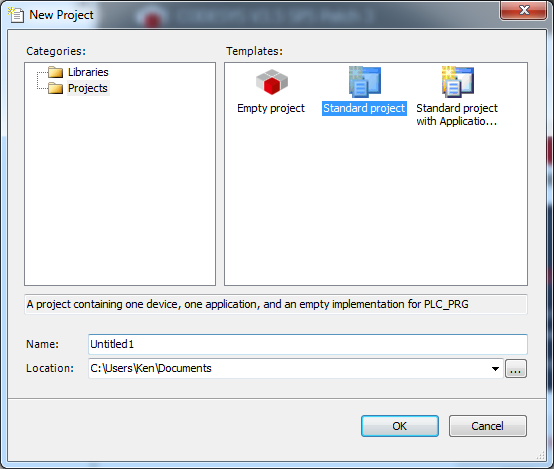
\includegraphics[width=350px]{img2.PNG}
	\end{center}
\caption{Project creation}
\label{fig:creation}
\end{figure}

CoDeSys will then ask you to choose tour device, since we are going to use simulation, we let the default value of ``Control Win V3".
Meanwhile, we change the value of the language for PLC\_PRG.
CoDeSys supports all languages described by the standard IEC-61131:

\begin{itemize}
\item Textual Languages:
\begin{itemize}
\item Instruction List (IL)
\item Structured Text (ST)
\end{itemize}
\item Grafic Languages:
\begin{itemize}
\item Sequential Function Chart (SFC) (Grafcet)
\item Function Block Diagram (FBD)
\item The Continuous Function Chart Editor (CFC)
\item Ladder Diagram (LD)
\end{itemize}
\end{itemize}

\begin{figure}[h!]
	\begin{center}
		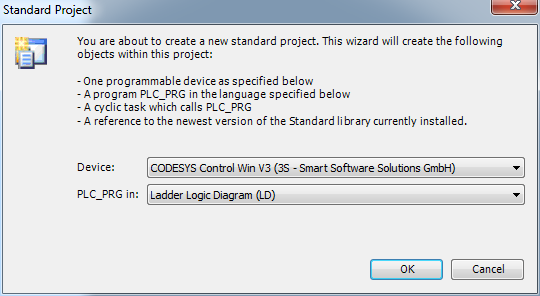
\includegraphics[width=300px]{img3.PNG}
	\end{center}
\caption{Language selection}
\label{fig:select}
\end{figure}

Once done, click on the PLC\_PRG file on the left, you will get a window similar to the one bellow I chose ladder for this example).

\begin{figure}[h!]
	\begin{center}
		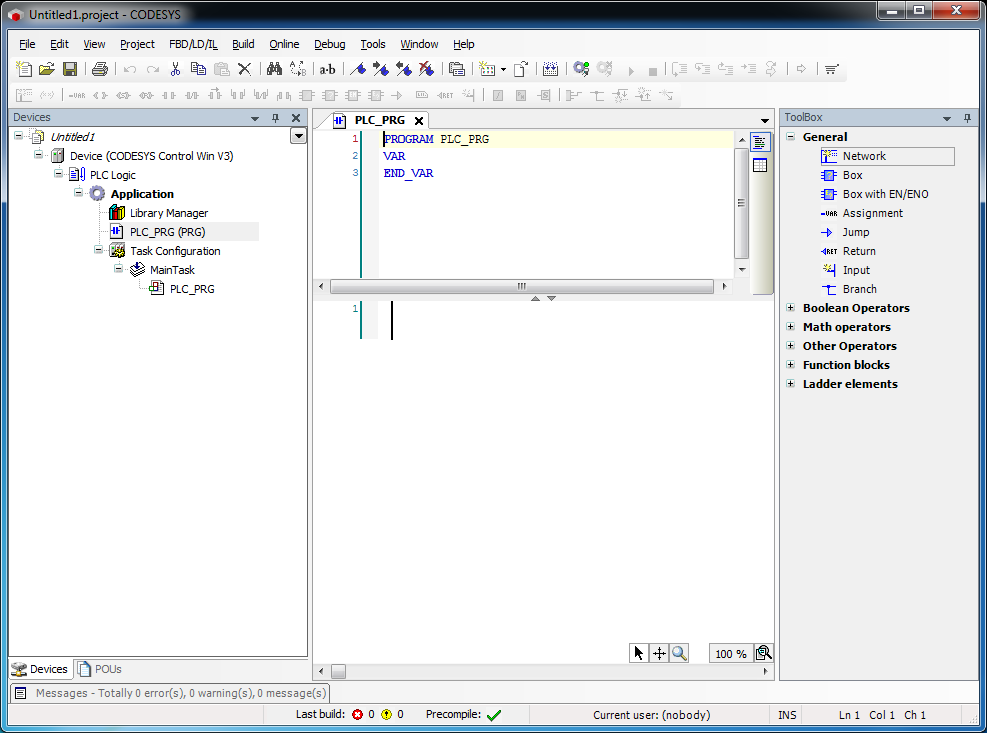
\includegraphics[width=350px]{img4.PNG}
	\end{center}
\caption{Main window}
\label{fig:main}
\end{figure}

Select the Application and right click on it or go to Project->Add object, and select Visualization.
This will create the environnement to run tour simulation with visual objects like buttons or lights.

We will start by creating a Global Variable List to simulate the inputs and outputs of a real system (as we don't actually have a PLC).\\
Right click on Application then Add object->Global Variable List.\\

You can now enter your inputs and outputs, the figure bellow gives an example.

\begin{figure}[h!]
	\begin{center}
		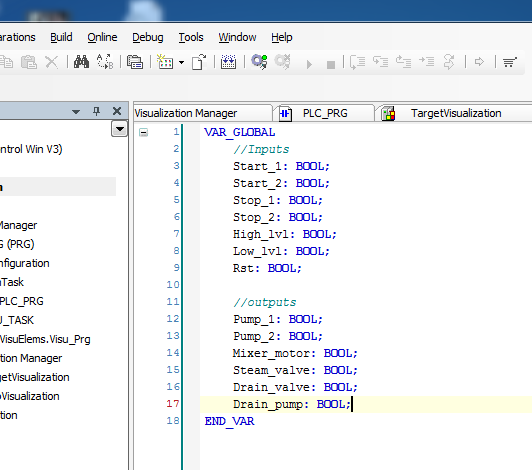
\includegraphics[width=300px]{img6.PNG}
	\end{center}
\caption{Global variables (I/Os)}
\label{fig:glob_var}
\end{figure}


\section{Variables}

\subsection{Syntax}
The syntax of the variables is such that their name can not contain the dot ``." character.
Past this detail, the grammar is as follows: \texttt{variable\_name: Type := value;}, the \texttt{value} part being facultative.

\subsection{Types}
See ``Data type" in the doc.


\section{Ladder programming}

Elements of for ladder programming are available in the right panel and on the top bar.
Local variables can be used to add intermediate variables that are not inputs or outputs (they are only usable in the current POU (program organization unit)). Here the POU is the PLC\_PRG file in ladder laguage.

\begin{figure}[h!]
	\begin{center}
		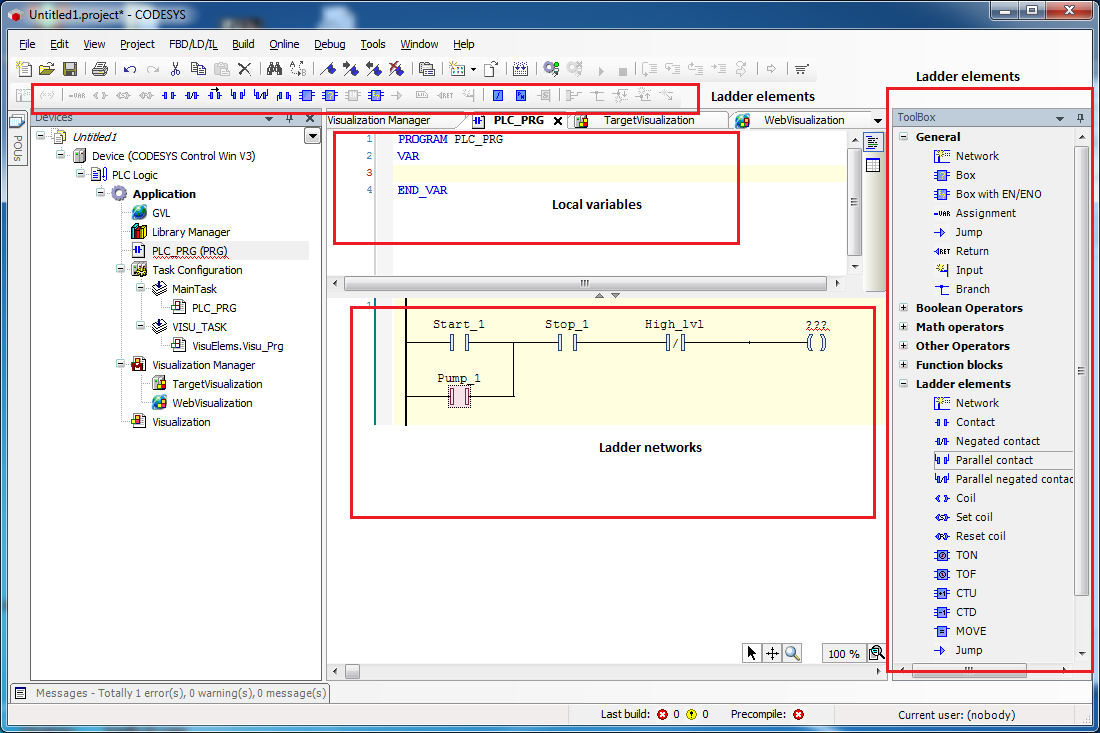
\includegraphics[width=350px]{img7.PNG}
	\end{center}
\caption{Network}
\label{fig:network}
\end{figure}

You can select variables to assign to the different elements of your network by clicking on the ``..." icon next to the name of the element (which is ``???" by default).
Then simply assign the variables by selecting them.
The same goes with local variables, both are available in this menu.

\begin{figure}[h!]
	\begin{center}
		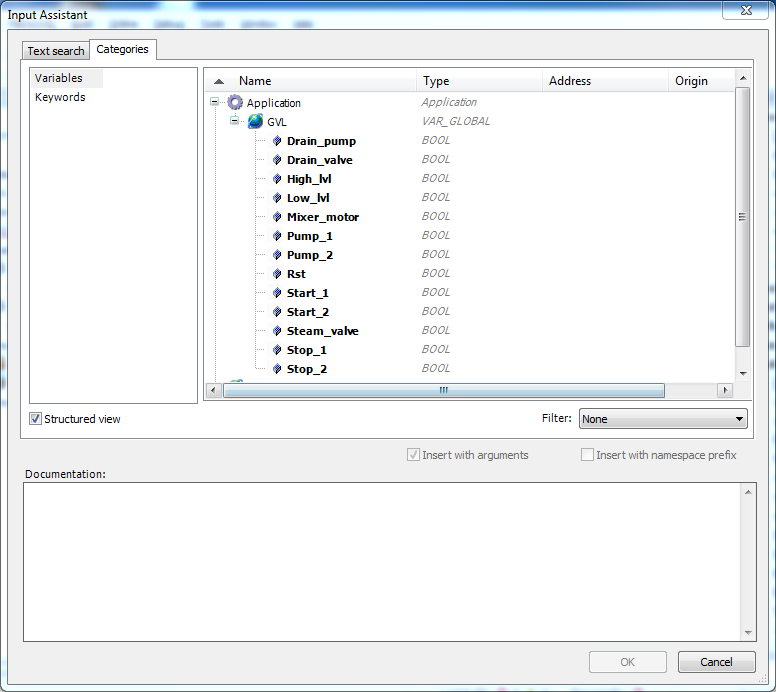
\includegraphics[width=250px]{img8.PNG}
	\end{center}
\caption{Selection}
\label{fig:sel}
\end{figure}

\paragraph{Edge detection}
Add a contact to your network, then right-click it and change it to ``Edge Detection" to get a rising edge detector.
Repeat the operation to have a falling edge detector.

\paragraph{Parallel branch}
In order to have a parallel branch that comes back up to the same output (see fig~\ref{fig:ladder-parallel}), you first need an element on the network.
Right-click it and choose Insert Contact Parallel.



% #######    ########      ###     #########   #######   #########  ##########
% ##         ##     ##    ## ##    ##         ##     ##  ##             ##
% ##         ##     ##   ##   ##   ##         ##         ##             ##
% ##   ####  ########   ##     ##  ######     ##         ######         ##
% ##     ##  ##   ##    #########  ##         ##         ##             ##
% ##     ##  ##    ##   ##     ##  ##         ##     ##  ##             ##
% ########   ##     ##  ##     ##  ##          #######   #########      ##

\section{Grafcet programming}

Elements of grafcet programming are available in the right panel as well as on the top bar.
Just like for ladder programming, local variables can be used to add intermediate variables that are not inputs or outputs (they are only usable in the current POU (program organization unit)). Here the POU is the PLC\_PRG file in grafcet laguage.

\begin{figure}[h!]
	\begin{center}
		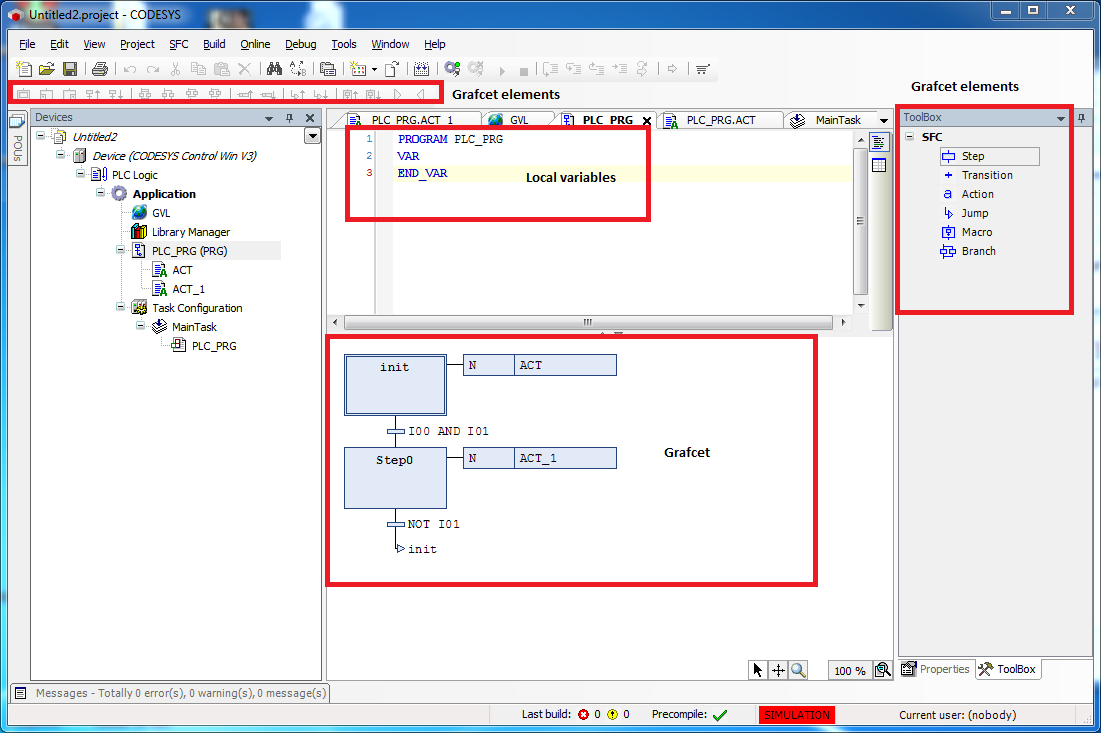
\includegraphics[width=350px]{img13.PNG}
	\end{center}
\caption{Grafcet}
\label{fig:grafcet}
\end{figure}

Once you've added some grafcet elements, you can create transition and actions to attach on it.
There are two ways of adding actions of transitions on a grafcet network : direct or indirect.\\
Direct adding means you write structured text logic expressions directly in the boxes (Transitions on \vref{fig:grafcet}).\\
Indirect adding means you have to create a transition or action file (right click on PLC\_PRG->Add object) in any format you want (ladder, structured text...) and detail your expressions for transitions or actions in this file.\\
For actions, a letter lets you choose whether you want you action the be delayed, time limited, etc... (the default choice is "N" : the action is active as long as the step is active).
See figure \vref{fig:tabgraf} for details on the different possibilities.

\begin{figure}[h!]
	\begin{center}
		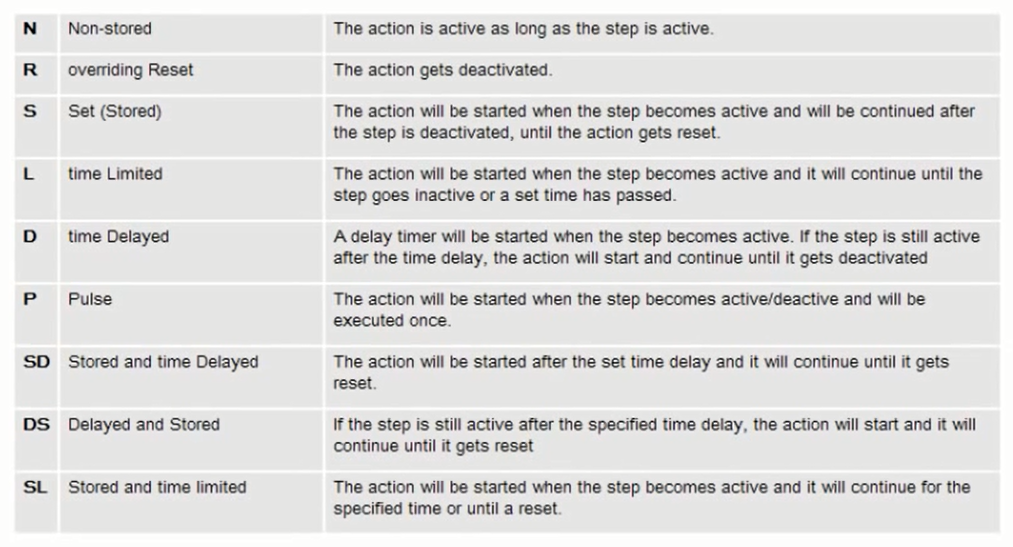
\includegraphics[width=300px]{tableaugrafcet.png}
	\end{center}
\caption{Action modes (``Qualifiers for Actions in SFC")}
\label{fig:tabgraf}
\end{figure}

Note that for the time-dependent actions, CodeSys is expecting a \texttt{TIME} variable next to the identifier.

Selection of variables is similar to the selection in ladder programming.

\subsection{Transition}
Several conditions can be concatenated in a single transition expression using \texttt{AND} and \texttt{OR}.

\paragraph{Timer}
A transition can be fired according to the time spent in the previous step (see fig~\ref{fig:transition-timer}).
To fire the transition after two seconds have been spent in the step \texttt{step0}, you would write:
\begin{verb}
  step0.t > t#2s
\end{verb}

\begin{figure}
  \begin{center}
    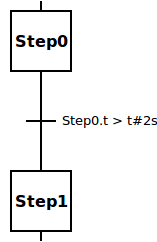
\includegraphics[height=5cm]{transition-timer.png}
  \end{center}
  \caption{The transition will be fired after 2 seconds have been spent in \texttt{Step0}.}
  \label{fig:transition-timer}
\end{figure}

\subsection{Convergence and divergence}
Convergences and divergences are generated using the ``branch" tool.
To create an AND-divergence, select a step you want to be part of a branch, and create a left or right branch (either \textit{via} right-click or the toolbar).
To create an OR-divergence, do the same thing, but selecting a transition.

\subsection{Useful modules}
Several modules can be quite useful:
\begin{description}
  \item[CTU] Counter\footnote{A \texttt{WORD} is 16-bit long.}
  \item[TON] Timer
\end{description}

Note that to easily obtain the documentation to a specific module, right-click on it $\rightarrow$ ``browse" $\rightarrow$ ``Go to definition".




% #######   ########   ##       ##  ##     ##
% ##    ##     ##      ###     ###  ##     ##
% ##           ##      ## ## ## ##  ##     ##
% #######      ##      ##  ###  ##  ##     ##
%       ##     ##      ##       ##  ##     ##
% ##    ##     ##      ##       ##  ##     ##
% #######   ########   ##       ##   #######

\section{Simulation and visualization}
\subsection{Setup}
Select simulation from the dropdown menu "Online" so that it ends up checked.

\begin{figure}[h!]
	\begin{center}
		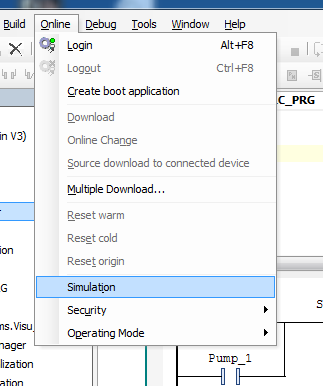
\includegraphics[width=150px]{img9.png}
	\end{center}
\caption{Selection}
\label{fig:simu}
\end{figure}

Then, from the same menu, select login. You are now in simulation mode (fig \vref{fig:simu_win})
There it is possible to start or stop the simulation by clicking on the "play" or "stop" button of the top bar.
It is also possible to assign (or force) values to variables by simply clicking several times on the variable. When your input variables have the wanted states go to Debug->Write(or Force) Value to assign (or force) the values to the system.\\
The network should response according to your inputs.

\begin{figure}[h!]
	\begin{center}
		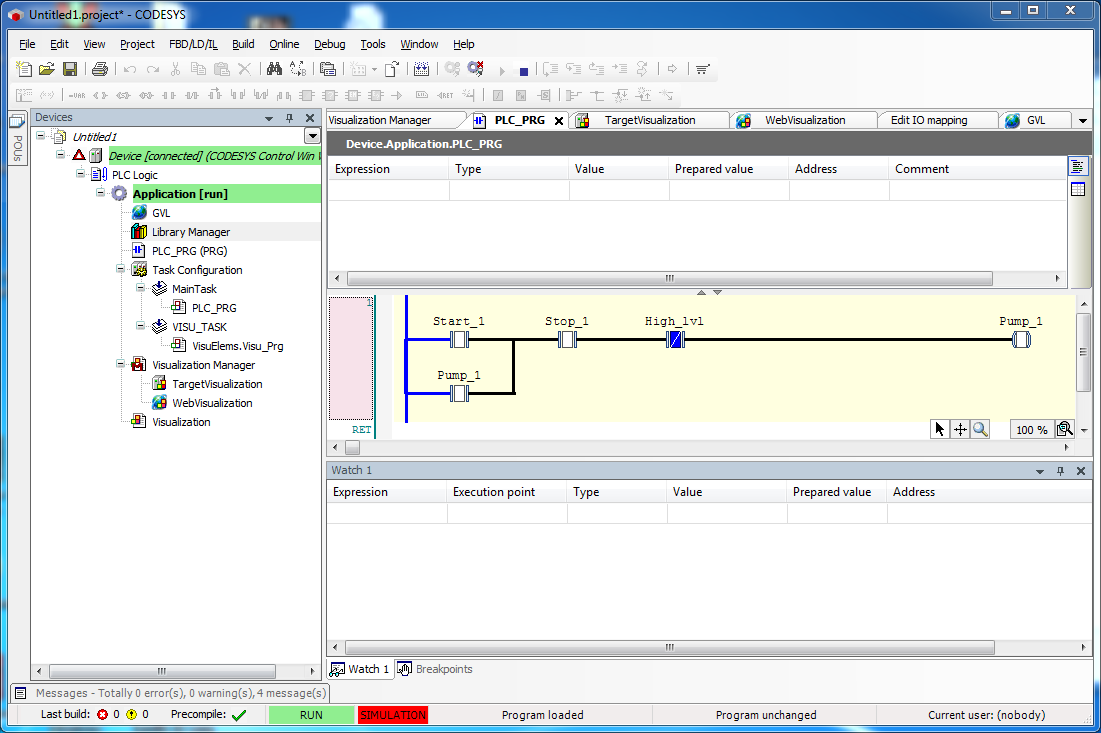
\includegraphics[width=300px]{img10.PNG}
	\end{center}
\caption{Simulation mode}
\label{fig:simu_win}
\end{figure}

\subsection{Visualization}

Double click on the Visualization you created during the setup of the project, you should get to the vizualization windows.\\
NB : The project needs to be ``Offline" to allow the modification of the visualization (Online->Logout in the top bar).\\
There you can add objects from the toolbox that can be linked to the different variables you created in your project (fig \vref{fig:prop})

\begin{figure}[h!]
	\begin{center}
		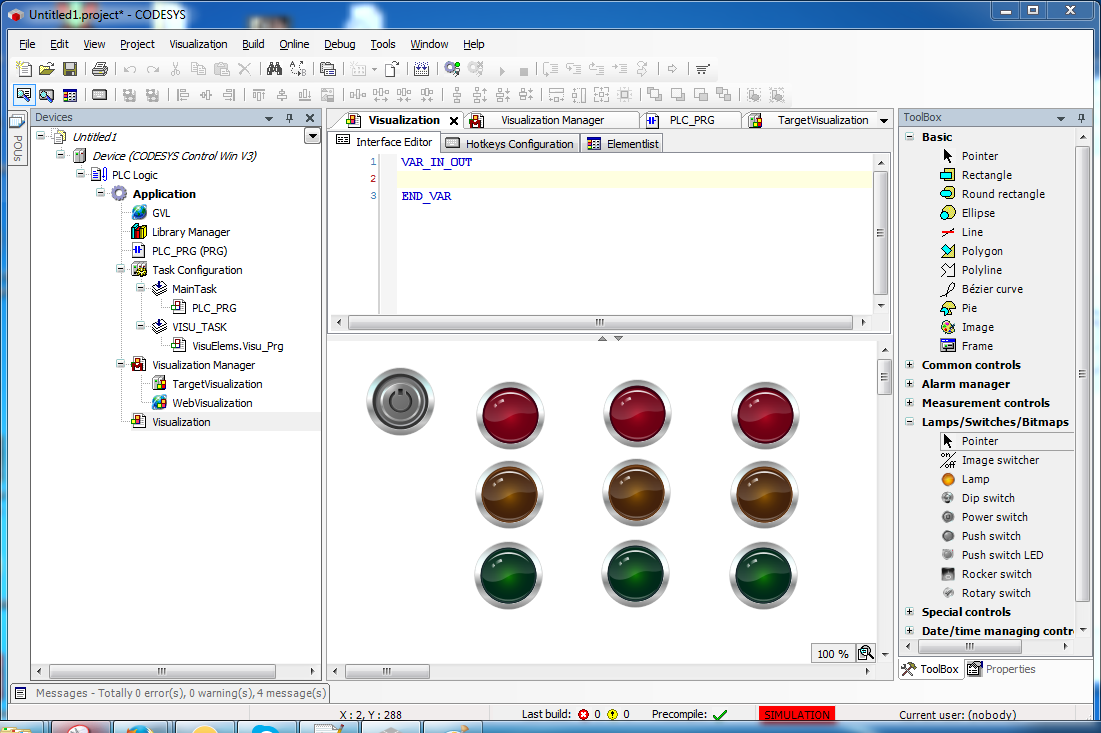
\includegraphics[width=300px]{img11.PNG}
	\end{center}
\caption{Visualization}
\label{fig:visu}
\end{figure}


\begin{figure}[h!]
	\begin{center}
		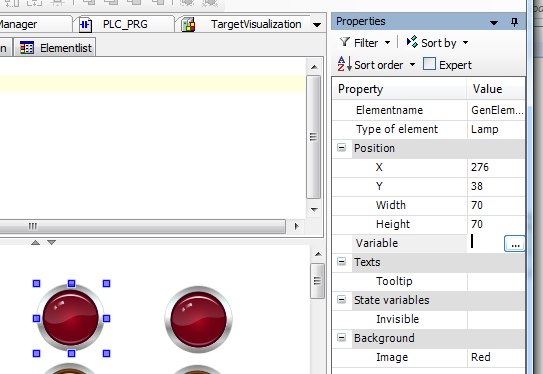
\includegraphics[width=150px]{img12.png}
	\end{center}
\caption{Properties}
\label{fig:prop}
\end{figure}

The visualization can then be used in sync with the simulation of the system by puting the project back online (Online->login menu in the top bar)

\subsubsection{Troubleshooting}
Should the simulation throw a ``License not found" error, it's probably because of the visualization.
Try removing the ``visualization manager" from the project tree, keeping only the ``visualization".
\end{document}

%\vref{fig:RISC}
